Table~\ref{tab:vf-ln-tax1-zcov} shows the mean loss ratios and corresponding coefficients of variation in the vulnerability function used in this test case.

When the exposure model and vulnerability model are provided to the OpenQuake classical PSHA-based hazard calculator, OpenQuake computes the hazard curves at the locations of the assets in the exposure model and at the specific intensity levels used in the vulnerability functions.

\begin{table}[htbp]

\centering
\tabcolsep=0.11cm
\scalebox{0.6}{

\begin{tabular}{ l c c c c c c c c c c c }

\hline
\rowcolor{anti-flashwhite}
\bf{PGA} & \bf{0.05g} & \bf{0.20g} & \bf{0.40g} & \bf{0.60g} & \bf{0.80g} & \bf{1.00g} & \bf{1.20g} & \bf{1.40g} & \bf{1.60g} & \bf{1.80g} & \bf{2.00g} \\
\hline
\bf{P.O.E.} & 3.896\times10^{-2} & 2.222\times10^{-2} & 8.171\times10^{-3} & 3.070\times10^{-3} & 1.230\times10^{-3} & 5.195\times10^{-4} & 2.254\times10^{-4} & 9.918\times10^{-5} & 4.353\times10^{-5} & 1.830\times10^{-5} & 6.925\times10^{-6} \\
\hline
\end{tabular}

}

\caption{Hazard curve for PGA at a single site}
\label{tab:hc-l1}
\end{table}

The intensity levels for the hazard curve are extracted from the vulnerability function: $[0.05, 0.20, 0.40, 0.60, 0.80, 1.00, 1.20, 1.40, 1.60, 1.80, 2.00]$. The hazard curve gives the probabilities of exceedance for a set of intensity levels within a specified time period. The time period in this case, $t_H$, is one year. The hazard curve at the location of the single asset used in this test case is shown in Table~\ref{tab:hc-l1}.

The probabilities of exceedance are: $[3.896\times10^{-2}, 2.222\times10^{-2}, 8.171\times10^{-3}, 3.070\times10^{-3}, 1.230\times10^{-3}, 5.195\times10^{-4}, 2.254\times10^{-4}, 9.918\times10^{-5}, 4.353\times10^{-5}, 1.830\times10^{-5}, 6.925\times10^{-6}]$. The probabilities of exceedance are first converted to annual rates (or frequencies) of exceedance by employing the Poissonion conversion:

\begin{equation}
	\lambda(iml) = \frac{-\ln [1 - prob(IML > iml, t_H)]}{t_H}
\end{equation}

The annual frequencies of exceedance are: $[3.974\times10^{2}, 2.247\times10^{2}, 8.205\times10^{3}, 3.075\times10^{3}, 1.231\times10^{3}, 5.197\times10^{4}, 2.254\times10^{4}, 9.918\times10^{5}, 4.353\times10^{5}, 1.829\times10^{5}, 6.925\times10^{6}]$.

The annual frequencies of occurrence are estimated by the differentiation of the annual frequencies of exceedance: $[1.727\times10^{2}, 1.426\times10^{2}, 5.130\times10^{3}, 1.845\times10^{3}, 7.109\times10^{4}, 2.942\times10^{4}, 1.262\times10^{4}, 5.565\times10^{5}, 2.524\times10^{5}, 1.137\times10^{5}]$.

The loss ratios at which the loss curve exceedance probabilities are calculated are obtained from the vulnerability function and the parameter `steps\_per\_interval'. The default value of `steps\_per\_interval' is one, which is the value used in this case. The loss ratios in the vulnerability function are $[0.01, 0.04, 0.10, 0.20, 0.33, 0.50, 0.67, 0.80, 0.90, 0.96, 0.99]$.

The vulnerability model is then transformed into a matrix describing probabilities of exceedance for the selected set of loss ratios conditional on the set of ground motion intensity levels. Since there is no variability in the loss ratio, calculation of the loss curves is straightforward in this case. Since the coefficients of variation in the vulnerability function are all zero, the lognormal distribution devolves into the degenerate distribution. The loss ratio exceedance matrix in this case is shown in Table~\ref{tab:lrem-ln-tax1-zcov}.

\begin{table}[htbp]

\centering
\begin{tabular}{ l c c c c c c c c c }

\hline
\rowcolor{anti-flashwhite}
\bf{LR | PGA} & \bf{0.05g} & \bf{0.20g} & \bf{0.40g} & \bf{0.60g} & \bf{0.80g} & \bf{1.00g} & \bf{1.20g} & \bf{\dots} & \bf{2.00g} \\
\hline
\bf{0.01} & 1 & 1 & 1 & 1 & 1 & 1 & 1 & \dots & 1 \\
\bf{0.04} & 0 & 1 & 1 & 1 & 1 & 1 & 1 & \dots & 1 \\
\bf{0.10} & 0 & 0 & 1 & 1 & 1 & 1 & 1 & \dots & 1 \\
\bf{0.20} & 0 & 0 & 0 & 1 & 1 & 1 & 1 & \dots & 1 \\
\bf{0.33} & 0 & 0 & 0 & 0 & 1 & 1 & 1 & \dots & 1 \\
\bf{0.50} & 0 & 0 & 0 & 0 & 0 & 1 & 1 & \dots & 1 \\
\bf{0.67} & 0 & 0 & 0 & 0 & 0 & 0 & 1 & \dots & 1 \\
\bf{0.80} & 0 & 0 & 0 & 0 & 0 & 0 & 0 & \dots & 1 \\
\bf{0.90} & 0 & 0 & 0 & 0 & 0 & 0 & 0 & \dots & 1 \\
\bf{0.96} & 0 & 0 & 0 & 0 & 0 & 0 & 0 & \dots & 1 \\
\bf{0.99} & 0 & 0 & 0 & 0 & 0 & 0 & 0 & \dots & 1 \\
\bf{1.00} & 0 & 0 & 0 & 0 & 0 & 0 & 0 & \dots & 0 \\
\hline
\end{tabular}

\caption{Conditional loss ratio exceedance matrix for classical risk test case 1a}
\label{tab:lrem-ln-tax1-zcov}
\end{table}

Now, the sum product of each row of the conditional loss ratio exceedance matrix with the annual frequencies of occurrence of the respective intensity levels gives the annual frequency of exceedance for the respective loss ratios. The loss ratio annual frequencies of exceedance thus calculated are: $[3.973\times10^{2}, 3.110\times10^{2}, 1.533\times10^{2}, 5.633\times10^{3}, 2.146\times10^{3}, 8.682\times10^{4}, 3.656\times10^{4}, 1.554\times10^{4}, 6.443\times10^{5}, 2.399\times10^{5}]$.

The probabilities of exceedance of the set of loss ratios are obtained by converting the frequencies of exceedance back into probabilities by using the Poissonion assumption. The loss curve probabilities of exceedance are: $[3.895\times10^{2}, 3.062\times10^{2}, 1.521\times10^{2}, 5.617\times10^{3}, 2.144\times10^{3}, 8.678\times10^{4}, 3.655\times10^{4}, 1.554\times10^{4}, 6.443\times10^{5}, 2.399\times10^{5}, 5.683\times10^{6}]$.

The loss curve thus calculated above is compared with the loss curve obtained using the OpenQuake classical PSHA based risk calculator in Figure~\ref{fig:lc-cr-1a}.

\begin{figure}[htbp]
\centering
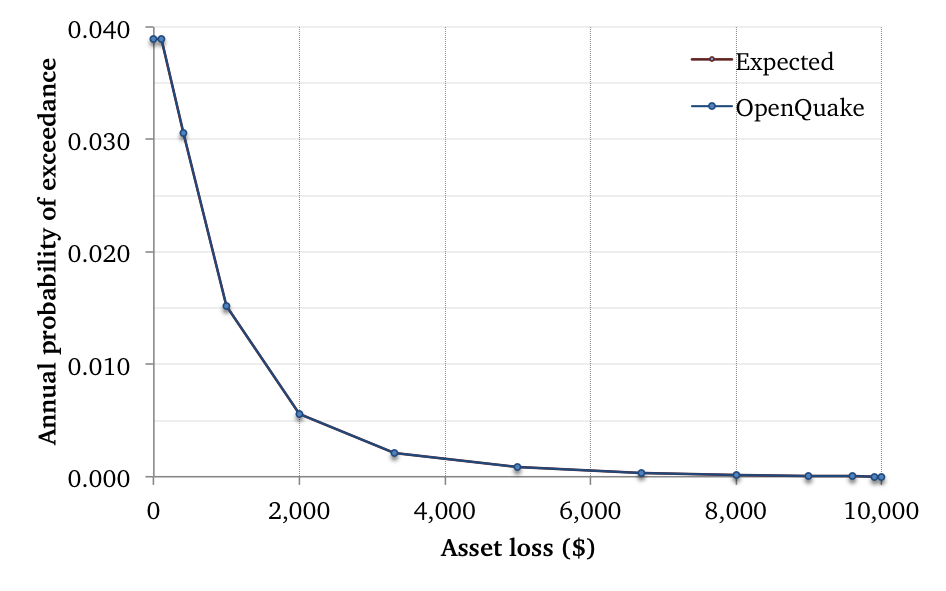
\includegraphics[width=12cm]{qareport/figures/fig-lc-cr-1a}
\caption{Loss curve comparison for classical risk test case 1a}
\label{fig:lc-cr-1a}
\end{figure}

The area under the annual loss exceedance curve gives the average annual loss. Table~\ref{tab:result-cr-1a} shows the comparison of the OpenQuake result for average annual loss with the expected result.
